\section{655 --- Print Binary Tree}
Print a binary tree in an $m\times n$ 2D string array following these rules:

\begin{enumerate}
\item The row number $m$ should be equal to the height of the given binary tree.
\item The column number $n$ should always be an odd number.
\item The root node's value (in string format) should be put in the exactly middle of the first row it can be put. The column and the row where the root node belongs will separate the rest space into two parts (\textbf{left-bottom part and right-bottom part}). You should print the left subtree in the left--bottom part and print the right subtree in the right--bottom part. The left-bottom part and the right-bottom part should have the same size. Even if one subtree is none while the other is not, you don't need to print anything for the none subtree but still need to leave the space as large as that for the other subtree. However, if two subtrees are none, then you don't need to leave space for both of them.
\item Each unused space should contain an empty string \lstinline[language=C++, basicstyle=\small\ttfamily, keywordstyle=\bfseries\color{green!40!black}]|""|.
\item Print the subtrees following the same rules.
\end{enumerate}

\paragraph{Example 1:}

\begin{flushleft}
\textbf{Input}:
\begin{figure}[H]
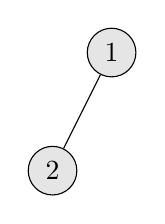
\begin{tikzpicture}
[every node/.style={draw, circle, fill=gray!20!, minimum size=5mm}]
\node{1}
child{node{2}}
child[missing];
\end{tikzpicture}
\end{figure}

\textbf{Output}:
\begin{lstlisting}[style=customc, caption={}]
{
["", "1", ""],
["2", "", ""]
}
\end{lstlisting}
\end{flushleft}

\paragraph{Example 2:}

\begin{flushleft}
\textbf{Input}:
\begin{figure}[H]
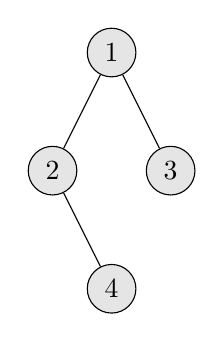
\begin{tikzpicture}
[every node/.style={draw, circle, fill=gray!20!, minimum size=5mm}]
\node{1}
child{node{2} child[missing] child{node{4}}}
child{node{3}};
\end{tikzpicture}
\end{figure}

\textbf{Output}:
\begin{lstlisting}[style=customc, caption={}]
[["", "", "", "1", "", "", ""],
 ["", "2", "", "", "", "3", ""],
 ["", "", "4", "", "", "", ""]]
\end{lstlisting}
\end{flushleft}

\paragraph{Example 3:}

\begin{flushleft}
\textbf{Input}:
\begin{figure}[H]
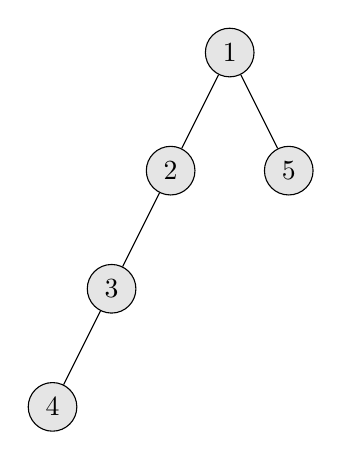
\begin{tikzpicture}
[every node/.style={draw, circle, fill=gray!20!, minimum size=5mm}]
\node{1}
child{node{2} child{ node{3} child{node{4}} child[missing] } child[missing]}
child{node{5}};
\end{tikzpicture}
\end{figure}
 
\textbf{Output}:
\begin{lstlisting}[style=customc, caption={}]
[["",  "",  "", "",  "", "", "", "1", "",  "",  "",  "",  "", "", ""]
 ["",  "",  "", "2", "", "", "", "",  "",  "",  "",  "5", "", "", ""]
 ["",  "3", "", "",  "", "", "", "",  "",  "",  "",  "",  "", "", ""]
 ["4", "",  "", "",  "", "", "", "",  "",  "",  "",  "",  "", "", ""]]d
\end{lstlisting}
\end{flushleft}

\textbf{Note}: 
\begin{itemize}
\item The height of binary tree is in the range of \lstinline[language=C++, basicstyle=\small\ttfamily, keywordstyle=\bfseries\color{green!40!black}]|[1, 10]|. 
\end{itemize}

\subsection{Divide And Conquer}
We need to get the height of the binary tree first, say $h$. The output matrix dimension will be $h\times (2^h-1)$. Then we go to the recursion process to put each node's value into the output matrix.
\begin{enumerate}
\item The recursive function will take current row, $r$, current size of columns $\ell$, and the start column $c$.
\item We put current node at the center of current row by considering the start column, i.e, $M[r][c + \ell/2]$.
\item Then we put left child of current node at next row with half of $l$, i.e, $M[r+1][c+\ell/4]$.
\item Next, we put right child of current node at next row with half of $l$ but the start column is $c+\ell/2+1$, i.e., $M[r+1][c+\ell/2+1+\ell/4]$
\item Go to step 1 to continue the recursive process. 
\end{enumerate}